\section{GUID Partition Table}
\label{sec:structure}
In diesem Abschnitt wird der Standard \textit{GUID Partition Table} (GPT) detailliert beschrieben.

Im Zuge dieser Ausarbeitung wurde außerdem eine Anwendung entwickelt, um Partitions-Informationen aus einem Datenträger, der nach dem GPT-Verfahren partitioniert ist, auszulesen.
Der komplette Quellcode ist im Github-Repository \textit{Nikos410/simple-gpt-reader}\footnote{\url{https://github.com/Nikos410/simple-gpt-reader}} zu finden.
Diese Anwendung wird im folgenden als \textit{simple-gpt-reader} bezeichnet.


\subsection{Aufbau}
Die einzelnen Datenstrukturen, die auf einem Datenträger vorliegen, der nach dem GPT-Verfahren partioniert ist, werden im folgenden genauer erläutert.
Diese Anordnung dieser Datenstrukturen ist in Abbildung \ref{fig:gpt_layout} grafisch dargestellt.

\begin{figure}[ht]
    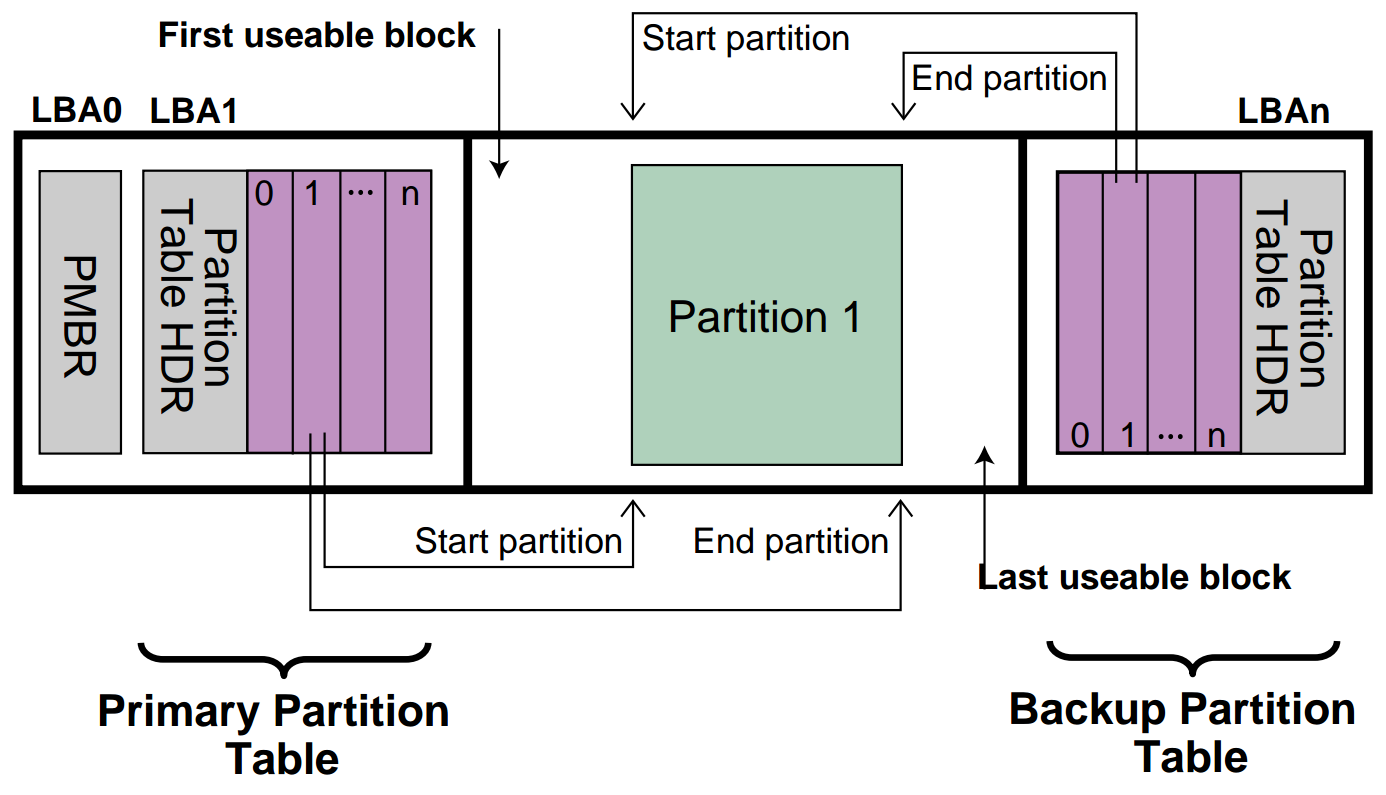
\includegraphics[width=\textwidth]{content/graphics/GPT_Layout.png}
    \caption{Datenstrukturen auf einem Datenträger mit GPT-Partitionierung. \cite{uefi-spec}}
    \label{fig:gpt_layout}
\end{figure}

\subsubsection{Protective MBR}
Viele ältere Betriebssyteme und Programme, die GPT nicht unterstützen, erwarten in LBA 0 einen MBR.
Wenn dieser nicht vorhanden ist, gilt der Datenträger für diese Systeme als nicht oder fehlerhaft partitioniert.
Damit der Datenträger in diesen Fällen nicht überschrieben wird, sieht GPT in LBA 0 einen MBR vor.

Dieser MBR gibt an, dass der Datenträger eine einzelne Partition beinhaltet, der den ganzen Datenträger umfasst.\footnote{
    Bei einem Datenträger, der die maximale von MBR adressierbare Größe überschreitet, beträgt die Größe dieser Partition die maximale Größe, die von MBR adressiert werden kann.
}
Dadurch muss in den zuvor erwähnten Systemen meist ein Nutzer zunächst diese Partitionen explizit löschen, bevor der Datenträger neu partitioniert werden kann.
Da so die GPT-Partitionsdaten sozusagen "geschützt" werden, wird dieser MBR als \textit{Protective MBR} bezeichnet.
Für die Funktion von GPT hat der Protective MBR ansonsten keine Bedeutung.

In Abbildung \ref{fig:protective-mbr} ist der Aufbau eines Datenträgers mit Protective MBR grafisch dargestellt.

\begin{figure}[ht]
    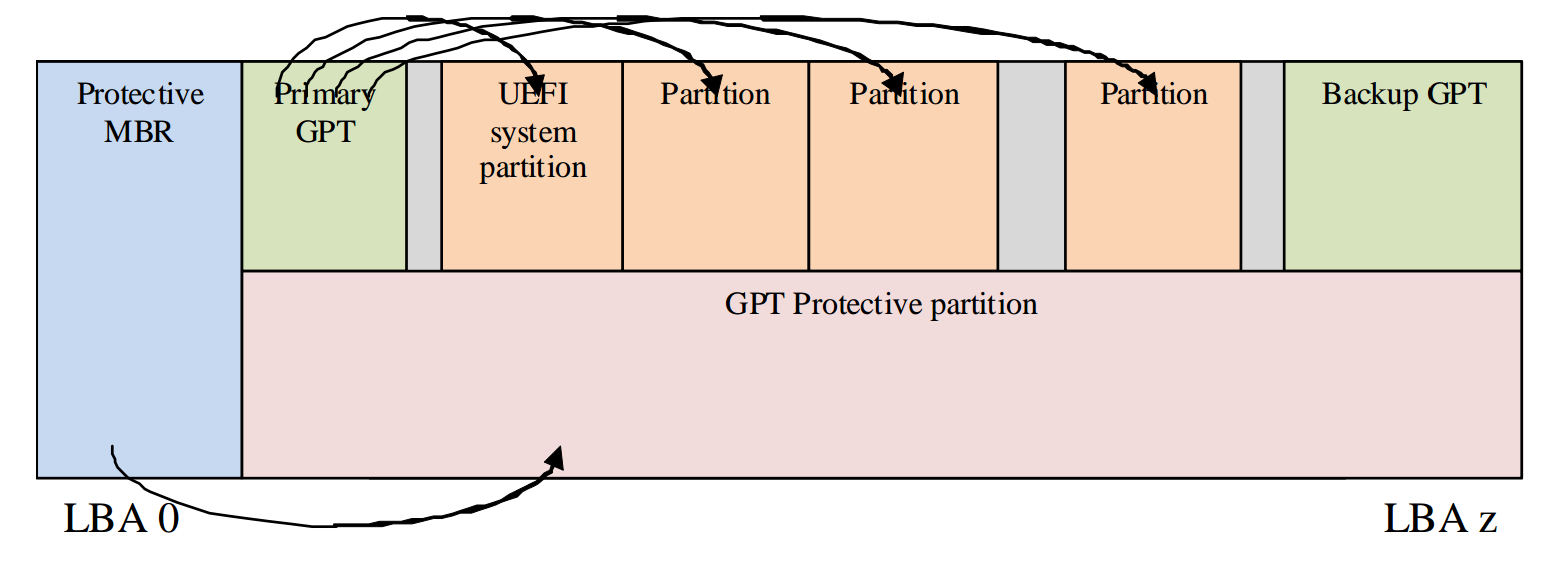
\includegraphics[width=\textwidth]{content/graphics/GPT_Layout_with_protective_MBR.png}
    
    \caption{Datenträger mit Protective MBR. \cite{uefi-spec}}
    \label{fig:protective-mbr}
\end{figure}


\subsubsection{GPT Header}
In LBA 1 befindet sich der sogenannte \textit{GPT Header}.
Dieser Header beinhaltet allgemeine Informationen über den Datenträger.
Im letzten Block eines Datenträgers befindet sich ein zweiter Header, um durch Redundanz Datenverlust vorzubeugen.
Der Header in LBA 1 wird dabei als \textit{primärer}, der Header am Ende als \textit{backup} Header bezeichnet.

In Abbildung \ref{fig:GptHeader.hpp} ist die Datenstruktur dargestellt, die im \textit{simple-gpt-reader} verwendet wird, um den Header abzubilden.
Die Bedeutung und der Zweck der einzelnen Felder werden im Folgenden genauer erläutert.

\begin{figure}[ht]
    \inputminted[baselinestretch=1.2, linenos, tabsize=4, breaklines, frame=single]{c++}{content/code/simple-gpt-reader/GptHeader.hpp}
    
    \caption{simple-gpt-reader/GptHeader.hpp (Auszug)}
    \label{fig:GptHeader.hpp}
\end{figure}

\newpage
\begin{itemize}
    \item \textbf{signature}: 
    Das erste Feld beinhaltet eine Signatur, um zu erkennen, ob es sich um einen GPT Header handelt.
    Diese Signatur muss den Wert \texttt{0x5452415020494645}\footnote{
        Dieser Wert entspricht dem ASCII-String "\texttt{EFI PART}"
    } 
    besitzen, damit es sich um einen gültigen GPT Header handelt.

    \item \textbf{revision}:
    Damit der GPT-Standard in Zukunft erweitert werden kann, ist hier die Revision gespeichert, an der man erkennen kann, wie die Daten im folgenden aufgebaut sind.
    In dieser Ausarbeitung ist die aktuellste\footnote{
        Stand Dezember 2020
    }
    Revision 1.0 beschrieben, in der dieses Feld den Wert \texttt{0x00010000} besitzt.

    \item \textbf{headerSize}:
    Die Größe des Headers in Bytes.
    Auch dies erleichtert es, den GPT-Standard in Zukunft erweitern zu können.

    \item \textbf{headerCrc32}:
    Die CRC32-Checksumme des Headers.
    Die Bytes, die für die Berechnung verwendet werden, ergeben sich aus dem Wert des Feldes \textit{headerSize}.
    Es wird diese Anzahl Bytes ab dem Anfang des Headers verwendet.
    Bei der Berechnung wird dieses Feld auf 0 gesetzt, damit der Wert dieses Feldes keinen Einfluss auf die Checksumme hat.

    \item \textbf{reserved}:
    Dieses Feld wird nicht verwendet und muss den Wert 0 besitzen. Zukünftige Revisionen können dieses Feld verwenden.

    \item \textbf{myLba}:
    Der Block, in dem sich der aktuelle Header befindet.

    \item \textbf{alternateLba}:
    Der Block, in dem sich der andere Header befindet.
    Beim primären Header besitzt beinhaltet Feld die Block-Nummer des Backup-Headers, beim Backup-Header die Block-Nummer des primären Headers.

    \item \textbf{firstUsableLba}:
    Der erste Block, der für eine Partition verwendet werden kann.

    \item \textbf{lastUsableLba}:
    Der letzte Block, der für eine Partition verwendet werden kann.

    \item \textbf{diskGuid}:
    Eine GUID, die verwendet werden kann, um den Datenträger eindeutig zu identifizieren.\cite{uefi-spec}
    Diese GUID wird beim Anlegen einer GPR-Partitionstabelle erstellt, daher kann nur die Partitionstabelle eindeutig identifiziert werden, weshalb die Bezeichnung \textit{diskGuid} irreführend ist.

    \item \textbf{partitionEntryLba}:
    Der erste Block des Partitions-Arrays. (vgl. Abschnitt \ref{sec:gpt:structure:entry-array})

    \item \textbf{numberOfPartitionEntries}:
    Die Anzahl der Einträge im Partitions-Array.
    Dies entspricht nicht der Anzahl der Partitionen, die tatsächlich auf dem Datenträger vorliegen, sondern der maximalen Anzahl der Partitionen, die im Partitions-Array gespeichert werden können.

    \item \textbf{sizeOfPartitionEntry}:
    Die Größe eines einzelnen Eintrages im Partitions-Array in Bytes.
    Zusammen mit \textit{numberOfPartitionEntries} kann so die Größe des Partitions-Arrays bestimmt werden.

    \item \textbf{partitionEntryArrayCrc32}:
    Die CRC32-Checksumme des Partitions-Arrays.
    
\end{itemize}

Der Rest des Blocks muss den Wert 0 besitzen.

\subsubsection{Partitions-Array}
\label{sec:gpt:structure:entry-array}
Im Partitions-Array werden die Informationen zu den einzelnen Partitionen gespeichert.
Auch von dieser Datenstruktur gibt es eine primäre und ein Backup.
Der primäre Header verweist im Feld \textit{partitionEntryLba} auf das primären Partitions-Array, der Backup-Header auf das Backup-Partitions-Array.

In Abbildung \ref{fig:GptPartitionEntry.hpp} ist die Datenstruktur dargestellt, die im \textit{simple-gpt-reader} verwendet wird, um ein Element im Partitions-Array abzubilden.
Die Bedeutung und der Zweck der einzelnen Felder werden im Folgenden genauer erläutert.

\begin{figure}[ht]
    \inputminted[baselinestretch=1.2, linenos, tabsize=4, breaklines, frame=single]{c++}{content/code/simple-gpt-reader/GptPartitionEntry.hpp}
    
    \caption{simple-gpt-reader/GptPartitionEntry.hpp (Auszug)}
    \label{fig:GptPartitionEntry.hpp}
\end{figure}

\begin{itemize}
    \item \textbf{partitionTypeGuid}:
    Eine GUID, die den Partitions-Typen angibt.
    Damit ist nicht das verwendete Dateisystem gemeint, sondern der Verwendungszweck der Partition.
    Beispielsweise verwendet Linux GUIDs um zwischen einfache nDaten-Partitionen, RAID-Partitionen oder Swap-Partitionen(Auslagerungsspeicher) zu unterscheiden.
    
    Da GUIDs als global eindeutig angesehen werden können, kann ein Betriebssystem-Hersteller selbstständig neue GUIDs vergeben, ohne diese bei einer zentralen Registrierungsstelle eintragen zu lassen.
    Daher gibt es auch keine vollständige Liste aller existierenden GUIDs, ein Betriebssystem kennt meist nur seine "eigenen" GUIDs.

    \item \textbf{uniquePartitionGuid}:
    Eine GUID, die diesen Partitions-Eintrag eindeutig identifiziert.

    \item \textbf{startingLba}:
    Der erste Block dieser Partition.

    \item \textbf{endingLba}:
    Der letzte Block dieser Partition.

    \item \textbf{attributes}:
    
    \item \textbf{partitionName}:
    Null-terminierter String, der einen Namen der Partition beinhaltet.
    Dieser Name muss nicht dem Namen des Dateisystems, das sich in dieser Partition befindet, entsprechen.

\end{itemize}

Wenn der Wert des Feldes \textit{sizeOfPartitionEntry} größer ist als die zuvor beschriebene Datenstruktur, muss der Rest des Partitions-Eintrags den Wert 0 besitzen und darf nicht anderweitig verwendet werden.\cite{uefi-spec}

\subsection{Bootloader}


\subsection{Vorteile gegenüber MBR}
\label{sec:gpt:advantages}

\begin{itemize}
    \item \textbf{Eindeutige Identifizierung von Partitionen:} 
    GPT versieht jede Partition mit einer GUID, um sie eindeutig identifizieren zu können.
    Bei GPT werden Partitionen durch ihre Partition auf dem Datenträger identifiziert (beispielsweise "Partition 2").
    Dies kann zu Problemen führen. 
    Wenn beispielsweise die erste Partition auf einem Datenträer in 2 Partitionen aufgeteilt wird, erhöht sich auch die Partitions-"Nummer" der darauf folgenden Partitionen (beispielsweise wird Partition 2 zu Partition 3).

    \item \textbf{Maximale Größe von Partitionen:}
    MBR speichert die LBA-Adresse des ersten Blocks und die Länge einer Partition mit 32 Bit großen Integer-Werten.
    Bei 512 Byte großen Blöcken ergibt sich so eine maximale Partitionsgröße von $ 2^{32} \cdot 512 \mathrm{B} = 2 \mathrm{TiB} $.

    In den meisten Betriebssystemen entspricht dies auch der maximalen Größe, die ein Datenträger besitzen kann.
    Da MBR (bei LBA-Adressierung) zusätzlich zur Block-Nummer des letzten Blockes einer Partition auch dessen Länge in Blöcken speichert, können in manchen Betriebssystemen bis zu 4TiB eines Datenträgers verwendet werden. 
    Um dies zu erreichen, kann eine 2TiB große Partition angelegt werden, dessen Startblock sich an der größten möglichen LBA-Adresse befindet.
    Dieses Verfahren wird allerdings nur von wenigen Betriebssystemen unterstützt, die intern Block-Nummern verwalten können, die größer als 32 Bit sind.
    Diese Betriebssysteme können meist auch das GPT verwenden, weshalb dieses Verfahren in der Praxis selten angewendet wird.\cite{mbr-4tb-workaround}

    Für heutige Datenträger sind oft weder 2TiB noch 4TiB ausreichend.
    GPT verwendet stattdessen 64 Bit große Datenstrukturen um Anfang und Ende einer Partition zu speichern, wodurch sich bei 512 Byte großen Blöcken eine maximale Größe von $ 2^{64} \cdot 512 \mathrm{B} = 8 \mathrm{ZiB} $ ergibt.

    \small
    \textit{
    TODO: Evtl. hier noch sagen, dass diese Limits voraussichtlich für die Zukunft ausreichend sind.
    Da müsste ich mir noch überlegen auf welcher Datengrundlage ich das Begründe.
    Ne Idee wäre diese Grafik zu verwenden: \url{https://upload.wikimedia.org/wikipedia/commons/9/90/Hard_drive_capacity_over_time.svg}
    Ist aber ne logarithmische Skala, das hochzurechnen wann das 144 PB erreicht wird frickelig.
    }

    \item \textbf{Maximale Anzahl von Partitionen:}
    Während MBR nur 4 primäre Partitionen unterstützt, kann GPT $ 2^{32} $ Partitionen verwalten.
    Dieses Limit wird allerdings nicht von allen Betriebssystemen unterstützt, beispielsweise können unter Linux maximal 256 Partionen und unter Windows 128 Partitionen auf einem Datenträger verwendet werden.

    \item \textbf{Erweiterbarkeit:} Version und Größe der Datenstrukturen werden in der Partitionstabelle gespeichert, um zukünftige Erweiterungen vornehmen zu können.

    \item \textbf{Datensicherheit:} GPT verwaltet 2 redundante Partitionstabellen in verschiedenen Bereichen eines Datenträgers.
    Außerdem werden CRC32 Checksummen verwendet um die Integrität der Daten sicherzustellen.

\end{itemize}
